\section{Actividad 1: Tansistor en zona de corte}

\subsection{Actividad de Simulación}

Para la simulacion implementamos el circuito presente

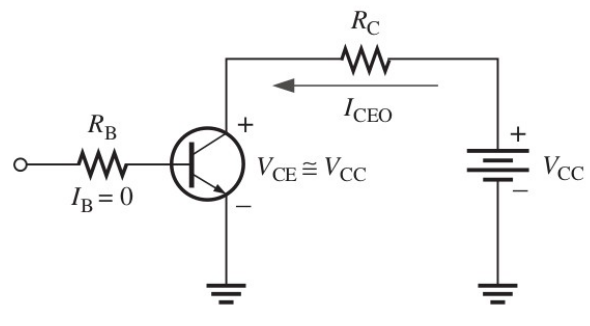
\includegraphics[width=6cm]{./imagenes/Circuito1.png}

Al no tener una fuente de voltaje en la base, el objetivo de la simulacion es medir la corriente de fuga $I_{CE0}$

\subsection{Materiales usados:}

\begin{itemize}
    \item Transistor NPN BC548A/B/C
    \item $R_B$ de 10k~$\Omega$
    \item $R_C$ de 1k~$\Omega$
    \item $V_{CC}$ de 10V
\end{itemize}

\subsection{Gráfico}

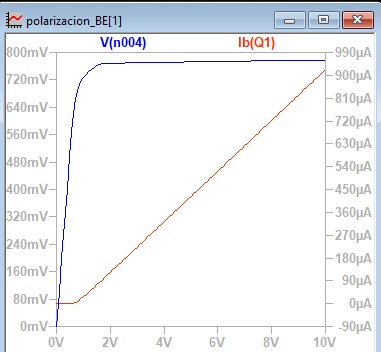
\includegraphics[width=8cm]{./imagenes/Grafico1.jpg}

\subsection{Conclusiones}

Contestando a la pregunta presentada para esta parte del trabajo, podemos observar que la corriente de fuga $I_{CE0}$ es muy pequeña, del orden de los nanoamperios, por lo que no podemos hacer la misma medición en el laboratorio, ya que los instrumentos de medición no tienen la precisión suficiente para medir corrientes tan pequeñas. 

